\documentclass[twoside]{book}

% Packages required by doxygen
\usepackage{fixltx2e}
\usepackage{calc}
\usepackage{doxygen}
\usepackage[export]{adjustbox} % also loads graphicx
\usepackage{graphicx}
\usepackage[utf8]{inputenc}
\usepackage{makeidx}
\usepackage{multicol}
\usepackage{multirow}
\PassOptionsToPackage{warn}{textcomp}
\usepackage{textcomp}
\usepackage[nointegrals]{wasysym}
\usepackage[table]{xcolor}

% Font selection
\usepackage[T1]{fontenc}
\usepackage[scaled=.90]{helvet}
\usepackage{courier}
\usepackage{amssymb}
\usepackage{sectsty}
\renewcommand{\familydefault}{\sfdefault}
\allsectionsfont{%
  \fontseries{bc}\selectfont%
  \color{darkgray}%
}
\renewcommand{\DoxyLabelFont}{%
  \fontseries{bc}\selectfont%
  \color{darkgray}%
}
\newcommand{\+}{\discretionary{\mbox{\scriptsize$\hookleftarrow$}}{}{}}

% Page & text layout
\usepackage{geometry}
\geometry{%
  a4paper,%
  top=2.5cm,%
  bottom=2.5cm,%
  left=2.5cm,%
  right=2.5cm%
}
\tolerance=750
\hfuzz=15pt
\hbadness=750
\setlength{\emergencystretch}{15pt}
\setlength{\parindent}{0cm}
\setlength{\parskip}{3ex plus 2ex minus 2ex}
\makeatletter
\renewcommand{\paragraph}{%
  \@startsection{paragraph}{4}{0ex}{-1.0ex}{1.0ex}{%
    \normalfont\normalsize\bfseries\SS@parafont%
  }%
}
\renewcommand{\subparagraph}{%
  \@startsection{subparagraph}{5}{0ex}{-1.0ex}{1.0ex}{%
    \normalfont\normalsize\bfseries\SS@subparafont%
  }%
}
\makeatother

% Headers & footers
\usepackage{fancyhdr}
\pagestyle{fancyplain}
\fancyhead[LE]{\fancyplain{}{\bfseries\thepage}}
\fancyhead[CE]{\fancyplain{}{}}
\fancyhead[RE]{\fancyplain{}{\bfseries\leftmark}}
\fancyhead[LO]{\fancyplain{}{\bfseries\rightmark}}
\fancyhead[CO]{\fancyplain{}{}}
\fancyhead[RO]{\fancyplain{}{\bfseries\thepage}}
\fancyfoot[LE]{\fancyplain{}{}}
\fancyfoot[CE]{\fancyplain{}{}}
\fancyfoot[RE]{\fancyplain{}{\bfseries\scriptsize Generated by Doxygen }}
\fancyfoot[LO]{\fancyplain{}{\bfseries\scriptsize Generated by Doxygen }}
\fancyfoot[CO]{\fancyplain{}{}}
\fancyfoot[RO]{\fancyplain{}{}}
\renewcommand{\footrulewidth}{0.4pt}
\renewcommand{\chaptermark}[1]{%
  \markboth{#1}{}%
}
\renewcommand{\sectionmark}[1]{%
  \markright{\thesection\ #1}%
}

% Indices & bibliography
\usepackage{natbib}
\usepackage[titles]{tocloft}
\setcounter{tocdepth}{3}
\setcounter{secnumdepth}{5}
\makeindex

% Hyperlinks (required, but should be loaded last)
\usepackage{ifpdf}
\ifpdf
  \usepackage[pdftex,pagebackref=true]{hyperref}
\else
  \usepackage[ps2pdf,pagebackref=true]{hyperref}
\fi
\hypersetup{%
  colorlinks=true,%
  linkcolor=blue,%
  citecolor=blue,%
  unicode%
}

% Custom commands
\newcommand{\clearemptydoublepage}{%
  \newpage{\pagestyle{empty}\cleardoublepage}%
}

\usepackage{caption}
\captionsetup{labelsep=space,justification=centering,font={bf},singlelinecheck=off,skip=4pt,position=top}

%===== C O N T E N T S =====

\begin{document}

% Titlepage & ToC
\hypersetup{pageanchor=false,
             bookmarksnumbered=true,
             pdfencoding=unicode
            }
\pagenumbering{alph}
\begin{titlepage}
\vspace*{7cm}
\begin{center}%
{\Large Libxbee }\\
\vspace*{1cm}
{\large Generated by Doxygen 1.8.14}\\
\end{center}
\end{titlepage}
\clearemptydoublepage
\pagenumbering{roman}
\tableofcontents
\clearemptydoublepage
\pagenumbering{arabic}
\hypersetup{pageanchor=true}

%--- Begin generated contents ---
\chapter{Module Index}
\section{Modules}
Here is a list of all modules\+:\begin{DoxyCompactList}
\item \contentsline{section}{A\+T\+Command\+Options}{\pageref{group___a_t_command_options}}{}
\item \contentsline{section}{Diagnostic\+Commands}{\pageref{group___diagnostic_commands}}{}
\item \contentsline{section}{Coordinator}{\pageref{group___coordinator}}{}
\item \contentsline{section}{Router}{\pageref{group___router}}{}
\item \contentsline{section}{End\+Device}{\pageref{group___end_device}}{}
\end{DoxyCompactList}

\chapter{Hierarchical Index}
\section{Class Hierarchy}
This inheritance list is sorted roughly, but not completely, alphabetically\+:\begin{DoxyCompactList}
\item \contentsline{section}{libxbee\+:\+:Version}{\pageref{structlibxbee_1_1_version}}{}
\item \contentsline{section}{libxbee\+:\+:modules\+:\+:X\+B\+E\+E\+Pro\+S2\+:\+:X\+B\+E\+E\+Pro\+S2}{\pageref{classlibxbee_1_1modules_1_1_x_b_e_e_pro_s2_1_1_x_b_e_e_pro_s2}}{}
\item \contentsline{section}{libxbee\+:\+:X\+B\+E\+E\+Serial}{\pageref{classlibxbee_1_1_x_b_e_e_serial}}{}
\begin{DoxyCompactList}
\item \contentsline{section}{libxbee\+:\+:Xbee\+Chimera\+Serial}{\pageref{classlibxbee_1_1_xbee_chimera_serial}}{}
\end{DoxyCompactList}
\end{DoxyCompactList}

\chapter{Class Index}
\section{Class List}
Here are the classes, structs, unions and interfaces with brief descriptions\+:\begin{DoxyCompactList}
\item\contentsline{section}{\mbox{\hyperlink{structlibxbee_1_1_version}{libxbee\+::\+Version}} }{\pageref{structlibxbee_1_1_version}}{}
\item\contentsline{section}{\mbox{\hyperlink{classlibxbee_1_1_xbee_chimera_serial}{libxbee\+::\+Xbee\+Chimera\+Serial}} }{\pageref{classlibxbee_1_1_xbee_chimera_serial}}{}
\item\contentsline{section}{\mbox{\hyperlink{classlibxbee_1_1modules_1_1_x_b_e_e_pro_s2_1_1_x_b_e_e_pro_s2}{libxbee\+::modules\+::\+X\+B\+E\+E\+Pro\+S2\+::\+X\+B\+E\+E\+Pro\+S2}} }{\pageref{classlibxbee_1_1modules_1_1_x_b_e_e_pro_s2_1_1_x_b_e_e_pro_s2}}{}
\item\contentsline{section}{\mbox{\hyperlink{classlibxbee_1_1_x_b_e_e_serial}{libxbee\+::\+X\+B\+E\+E\+Serial}} }{\pageref{classlibxbee_1_1_x_b_e_e_serial}}{}
\end{DoxyCompactList}

\chapter{File Index}
\section{File List}
Here is a list of all documented files with brief descriptions\+:\begin{DoxyCompactList}
\item\contentsline{section}{{\bfseries xb\+\_\+chimera\+\_\+serial.\+hpp} }{\pageref{xb__chimera__serial_8hpp}}{}
\item\contentsline{section}{\mbox{\hyperlink{xb__definitions_8hpp}{xb\+\_\+definitions.\+hpp}} }{\pageref{xb__definitions_8hpp}}{}
\item\contentsline{section}{{\bfseries xb\+\_\+nodemcu\+\_\+serial.\+hpp} }{\pageref{xb__nodemcu__serial_8hpp}}{}
\item\contentsline{section}{{\bfseries xb\+\_\+serial.\+hpp} }{\pageref{xb__serial_8hpp}}{}
\item\contentsline{section}{modules/xbee\+\_\+pro\+\_\+s2/{\bfseries xbpros2.\+hpp} }{\pageref{xbpros2_8hpp}}{}
\end{DoxyCompactList}

\chapter{Module Documentation}
\hypertarget{group___a_t_command_options}{}\section{A\+T\+Command\+Options}
\label{group___a_t_command_options}\index{A\+T\+Command\+Options@{A\+T\+Command\+Options}}
\begin{DoxyCompactItemize}
\item 
\#define \mbox{\hyperlink{group___a_t_command_options_ga44b29b82d01677566af011179946866f}{X\+B\+\_\+\+C\+M\+D\+\_\+\+M\+O\+D\+E\+\_\+\+T\+I\+M\+E\+O\+UT}}~\char`\"{}CT\char`\"{}
\item 
\#define \mbox{\hyperlink{group___a_t_command_options_ga521bbb1db05244aa3171ddeacb3a528e}{X\+B\+\_\+\+C\+M\+D\+\_\+\+M\+O\+D\+E\+\_\+\+E\+X\+IT}}~\char`\"{}CN\char`\"{}
\item 
\#define \mbox{\hyperlink{group___a_t_command_options_ga87806745d2177177af3bc9da86cbdd2f}{X\+B\+\_\+\+S\+E\+T\+\_\+\+G\+U\+A\+R\+D\+\_\+\+T\+I\+ME}}~\char`\"{}GT\char`\"{}
\item 
\#define \mbox{\hyperlink{group___a_t_command_options_gaaa54d14d569183034d941ef1e82dc3e5}{X\+B\+\_\+\+S\+E\+T\+\_\+\+C\+M\+D\+\_\+\+S\+E\+Q\+\_\+\+C\+H\+AR}}~\char`\"{}CC\char`\"{}
\end{DoxyCompactItemize}


\subsection{Detailed Description}


\subsection{Macro Definition Documentation}
\mbox{\Hypertarget{group___a_t_command_options_ga521bbb1db05244aa3171ddeacb3a528e}\label{group___a_t_command_options_ga521bbb1db05244aa3171ddeacb3a528e}} 
\index{A\+T\+Command\+Options@{A\+T\+Command\+Options}!X\+B\+\_\+\+C\+M\+D\+\_\+\+M\+O\+D\+E\+\_\+\+E\+X\+IT@{X\+B\+\_\+\+C\+M\+D\+\_\+\+M\+O\+D\+E\+\_\+\+E\+X\+IT}}
\index{X\+B\+\_\+\+C\+M\+D\+\_\+\+M\+O\+D\+E\+\_\+\+E\+X\+IT@{X\+B\+\_\+\+C\+M\+D\+\_\+\+M\+O\+D\+E\+\_\+\+E\+X\+IT}!A\+T\+Command\+Options@{A\+T\+Command\+Options}}
\subsubsection{\texorpdfstring{X\+B\+\_\+\+C\+M\+D\+\_\+\+M\+O\+D\+E\+\_\+\+E\+X\+IT}{XB\_CMD\_MODE\_EXIT}}
{\footnotesize\ttfamily \#define X\+B\+\_\+\+C\+M\+D\+\_\+\+M\+O\+D\+E\+\_\+\+E\+X\+IT~\char`\"{}CN\char`\"{}}

Exit Command Mode Explicitly exit the module from AT command mode \mbox{\Hypertarget{group___a_t_command_options_ga44b29b82d01677566af011179946866f}\label{group___a_t_command_options_ga44b29b82d01677566af011179946866f}} 
\index{A\+T\+Command\+Options@{A\+T\+Command\+Options}!X\+B\+\_\+\+C\+M\+D\+\_\+\+M\+O\+D\+E\+\_\+\+T\+I\+M\+E\+O\+UT@{X\+B\+\_\+\+C\+M\+D\+\_\+\+M\+O\+D\+E\+\_\+\+T\+I\+M\+E\+O\+UT}}
\index{X\+B\+\_\+\+C\+M\+D\+\_\+\+M\+O\+D\+E\+\_\+\+T\+I\+M\+E\+O\+UT@{X\+B\+\_\+\+C\+M\+D\+\_\+\+M\+O\+D\+E\+\_\+\+T\+I\+M\+E\+O\+UT}!A\+T\+Command\+Options@{A\+T\+Command\+Options}}
\subsubsection{\texorpdfstring{X\+B\+\_\+\+C\+M\+D\+\_\+\+M\+O\+D\+E\+\_\+\+T\+I\+M\+E\+O\+UT}{XB\_CMD\_MODE\_TIMEOUT}}
{\footnotesize\ttfamily \#define X\+B\+\_\+\+C\+M\+D\+\_\+\+M\+O\+D\+E\+\_\+\+T\+I\+M\+E\+O\+UT~\char`\"{}CT\char`\"{}}

Command Mode Timeout Set/\+Read the period of inactivity (no valid commands received) after which the RF module automatically exits AT Command Mode and returns to Idle Mode.

Parameter Range\+: 2-\/0x028F \mbox{[}x100mS\mbox{]}~\newline
Parameter Default\+: 0x64 \mbox{[}100d\mbox{]} \mbox{\Hypertarget{group___a_t_command_options_gaaa54d14d569183034d941ef1e82dc3e5}\label{group___a_t_command_options_gaaa54d14d569183034d941ef1e82dc3e5}} 
\index{A\+T\+Command\+Options@{A\+T\+Command\+Options}!X\+B\+\_\+\+S\+E\+T\+\_\+\+C\+M\+D\+\_\+\+S\+E\+Q\+\_\+\+C\+H\+AR@{X\+B\+\_\+\+S\+E\+T\+\_\+\+C\+M\+D\+\_\+\+S\+E\+Q\+\_\+\+C\+H\+AR}}
\index{X\+B\+\_\+\+S\+E\+T\+\_\+\+C\+M\+D\+\_\+\+S\+E\+Q\+\_\+\+C\+H\+AR@{X\+B\+\_\+\+S\+E\+T\+\_\+\+C\+M\+D\+\_\+\+S\+E\+Q\+\_\+\+C\+H\+AR}!A\+T\+Command\+Options@{A\+T\+Command\+Options}}
\subsubsection{\texorpdfstring{X\+B\+\_\+\+S\+E\+T\+\_\+\+C\+M\+D\+\_\+\+S\+E\+Q\+\_\+\+C\+H\+AR}{XB\_SET\_CMD\_SEQ\_CHAR}}
{\footnotesize\ttfamily \#define X\+B\+\_\+\+S\+E\+T\+\_\+\+C\+M\+D\+\_\+\+S\+E\+Q\+\_\+\+C\+H\+AR~\char`\"{}CC\char`\"{}}

Command Sequence Character Set/\+Read the A\+S\+C\+II character value to be used between Guard Times of the AT Command Mode Sequence (GT + CC + GT). The AT Command Mode Sequence enters the RF module into AT Command Mode. The CC command is only supported when using AT firmware\+: 20xx (AT coordinator), 22xx (AT router), 28xx (AT end device)

Parameter Range\+: 0-\/0x\+FF~\newline
Parameter Default\+: 0x2B (\textquotesingle{}+\textquotesingle{} A\+S\+C\+II) \mbox{\Hypertarget{group___a_t_command_options_ga87806745d2177177af3bc9da86cbdd2f}\label{group___a_t_command_options_ga87806745d2177177af3bc9da86cbdd2f}} 
\index{A\+T\+Command\+Options@{A\+T\+Command\+Options}!X\+B\+\_\+\+S\+E\+T\+\_\+\+G\+U\+A\+R\+D\+\_\+\+T\+I\+ME@{X\+B\+\_\+\+S\+E\+T\+\_\+\+G\+U\+A\+R\+D\+\_\+\+T\+I\+ME}}
\index{X\+B\+\_\+\+S\+E\+T\+\_\+\+G\+U\+A\+R\+D\+\_\+\+T\+I\+ME@{X\+B\+\_\+\+S\+E\+T\+\_\+\+G\+U\+A\+R\+D\+\_\+\+T\+I\+ME}!A\+T\+Command\+Options@{A\+T\+Command\+Options}}
\subsubsection{\texorpdfstring{X\+B\+\_\+\+S\+E\+T\+\_\+\+G\+U\+A\+R\+D\+\_\+\+T\+I\+ME}{XB\_SET\_GUARD\_TIME}}
{\footnotesize\ttfamily \#define X\+B\+\_\+\+S\+E\+T\+\_\+\+G\+U\+A\+R\+D\+\_\+\+T\+I\+ME~\char`\"{}GT\char`\"{}}

Guard Times Set required period of silence before and after the Command Sequence Characters of the AT Command Mode Sequence (GT + CC + GT). The period of silence is used to prevent inadvertent entrance into AT Command Mode

Parameter Range\+: 1-\/0x0\+C\+E4 \href{max of 3.3 decimal sec}{\tt x1mS}~\newline
Parameter Default\+: 0x3\+E8 \mbox{[}1000d\mbox{]} 
\hypertarget{group___diagnostic_commands}{}\section{Diagnostic\+Commands}
\label{group___diagnostic_commands}\index{Diagnostic\+Commands@{Diagnostic\+Commands}}
\begin{DoxyCompactItemize}
\item 
\#define \mbox{\hyperlink{group___diagnostic_commands_ga604d8e87718a1dc53cded0e3c020fc40}{X\+B\+\_\+\+F\+I\+R\+M\+W\+A\+R\+E\+\_\+\+V\+ER}}~\char`\"{}VR\char`\"{}
\item 
\#define \mbox{\hyperlink{group___diagnostic_commands_ga58a2fc2812c3b0fd035f22391354ec16}{X\+B\+\_\+\+H\+A\+R\+D\+W\+A\+R\+E\+\_\+\+V\+ER}}~\char`\"{}HV\char`\"{}
\end{DoxyCompactItemize}


\subsection{Detailed Description}


\subsection{Macro Definition Documentation}
\mbox{\Hypertarget{group___diagnostic_commands_ga604d8e87718a1dc53cded0e3c020fc40}\label{group___diagnostic_commands_ga604d8e87718a1dc53cded0e3c020fc40}} 
\index{Diagnostic\+Commands@{Diagnostic\+Commands}!X\+B\+\_\+\+F\+I\+R\+M\+W\+A\+R\+E\+\_\+\+V\+ER@{X\+B\+\_\+\+F\+I\+R\+M\+W\+A\+R\+E\+\_\+\+V\+ER}}
\index{X\+B\+\_\+\+F\+I\+R\+M\+W\+A\+R\+E\+\_\+\+V\+ER@{X\+B\+\_\+\+F\+I\+R\+M\+W\+A\+R\+E\+\_\+\+V\+ER}!Diagnostic\+Commands@{Diagnostic\+Commands}}
\subsubsection{\texorpdfstring{X\+B\+\_\+\+F\+I\+R\+M\+W\+A\+R\+E\+\_\+\+V\+ER}{XB\_FIRMWARE\_VER}}
{\footnotesize\ttfamily \#define X\+B\+\_\+\+F\+I\+R\+M\+W\+A\+R\+E\+\_\+\+V\+ER~\char`\"{}VR\char`\"{}}

Firmware Version Read firmware version of the module. The firmware version returns 4 hexadecimal values (2 bytes) \char`\"{}\+A\+B\+C\+D\char`\"{}. Digits A\+BC are the main release number and D is the revision number from the main release. \char`\"{}\+B\char`\"{} is a variant designator.

X\+Bee and X\+Bee-\/\+P\+RO ZB modules return\+: 0x2xxx versions~\newline
X\+Bee and X\+Bee-\/\+P\+RO Z\+Net modules return\+: 0x1xxx versions~\newline
 Z\+Net firmware is not compatible with ZB firmware

Parameter Range\+: 0-\/0x\+F\+F\+FF \mbox{[}read-\/only\mbox{]}~\newline
Parameter Default\+: Factory Set \mbox{\Hypertarget{group___diagnostic_commands_ga58a2fc2812c3b0fd035f22391354ec16}\label{group___diagnostic_commands_ga58a2fc2812c3b0fd035f22391354ec16}} 
\index{Diagnostic\+Commands@{Diagnostic\+Commands}!X\+B\+\_\+\+H\+A\+R\+D\+W\+A\+R\+E\+\_\+\+V\+ER@{X\+B\+\_\+\+H\+A\+R\+D\+W\+A\+R\+E\+\_\+\+V\+ER}}
\index{X\+B\+\_\+\+H\+A\+R\+D\+W\+A\+R\+E\+\_\+\+V\+ER@{X\+B\+\_\+\+H\+A\+R\+D\+W\+A\+R\+E\+\_\+\+V\+ER}!Diagnostic\+Commands@{Diagnostic\+Commands}}
\subsubsection{\texorpdfstring{X\+B\+\_\+\+H\+A\+R\+D\+W\+A\+R\+E\+\_\+\+V\+ER}{XB\_HARDWARE\_VER}}
{\footnotesize\ttfamily \#define X\+B\+\_\+\+H\+A\+R\+D\+W\+A\+R\+E\+\_\+\+V\+ER~\char`\"{}HV\char`\"{}}

Hardware Version Read the hardware version of the module version of the module. This command can be used to distinguish among different hardware platforms. The upper byte returns a value that is unique to each module type. The lower byte indicates the hardware revision. X\+Bee ZB and X\+Bee Z\+Net modules return the following (hexadecimal) values\+:~\newline
0x19xx -\/ X\+Bee module~\newline
0x1\+Axx -\/ X\+Bee-\/\+P\+RO module

Parameter Range\+: 0-\/0x\+F\+F\+FF \mbox{[}read-\/only\mbox{]}~\newline
Parameter Default\+: Factory Set 
\hypertarget{group___coordinator}{}\section{Coordinator}
\label{group___coordinator}\index{Coordinator@{Coordinator}}

\hypertarget{group___router}{}\section{Router}
\label{group___router}\index{Router@{Router}}

\hypertarget{group___end_device}{}\section{End\+Device}
\label{group___end_device}\index{End\+Device@{End\+Device}}

\chapter{Class Documentation}
\hypertarget{structlibxbee_1_1_version}{}\section{libxbee\+:\+:Version Struct Reference}
\label{structlibxbee_1_1_version}\index{libxbee\+::\+Version@{libxbee\+::\+Version}}
\subsection*{Public Attributes}
\begin{DoxyCompactItemize}
\item 
\mbox{\Hypertarget{structlibxbee_1_1_version_ad2ebf2c33042396e9865b7eec460bf9e}\label{structlibxbee_1_1_version_ad2ebf2c33042396e9865b7eec460bf9e}} 
uint16\+\_\+t {\bfseries firmware\+Version}
\item 
\mbox{\Hypertarget{structlibxbee_1_1_version_a67ef00d03fbc2918b1f6b0380fc61650}\label{structlibxbee_1_1_version_a67ef00d03fbc2918b1f6b0380fc61650}} 
uint16\+\_\+t {\bfseries hardware\+Version}
\end{DoxyCompactItemize}


The documentation for this struct was generated from the following file\+:\begin{DoxyCompactItemize}
\item 
\mbox{\hyperlink{xb__definitions_8hpp}{xb\+\_\+definitions.\+hpp}}\end{DoxyCompactItemize}

\hypertarget{classlibxbee_1_1_xbee_chimera_serial}{}\section{libxbee\+:\+:Xbee\+Chimera\+Serial Class Reference}
\label{classlibxbee_1_1_xbee_chimera_serial}\index{libxbee\+::\+Xbee\+Chimera\+Serial@{libxbee\+::\+Xbee\+Chimera\+Serial}}
Inheritance diagram for libxbee\+:\+:Xbee\+Chimera\+Serial\+:\begin{figure}[H]
\begin{center}
\leavevmode
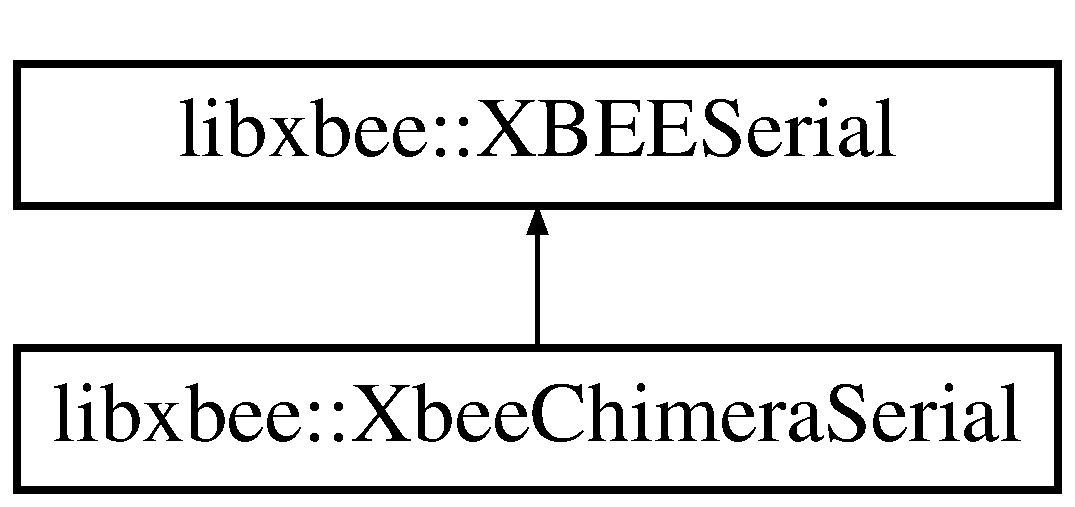
\includegraphics[height=2.000000cm]{classlibxbee_1_1_xbee_chimera_serial}
\end{center}
\end{figure}
\subsection*{Public Member Functions}
\begin{DoxyCompactItemize}
\item 
\mbox{\Hypertarget{classlibxbee_1_1_xbee_chimera_serial_a6b752002a4bc396f5c017d1288561fde}\label{classlibxbee_1_1_xbee_chimera_serial_a6b752002a4bc396f5c017d1288561fde}} 
void {\bfseries initialize} (Chimera\+::\+Serial\+::\+Baud\+Rate baud=Chimera\+::\+Serial\+::\+Baud\+Rate\+::\+S\+E\+R\+I\+A\+L\+\_\+\+B\+A\+U\+D\+\_\+115200, Chimera\+::\+Serial\+::\+Modes tx\+\_\+mode=Chimera\+::\+Serial\+::\+Modes\+::\+B\+L\+O\+C\+K\+I\+NG, Chimera\+::\+Serial\+::\+Modes rx\+\_\+mode=Chimera\+::\+Serial\+::\+Modes\+::\+B\+L\+O\+C\+K\+I\+NG)
\item 
\mbox{\Hypertarget{classlibxbee_1_1_xbee_chimera_serial_acd9fd19475ab2a11852c1ef1c67f693a}\label{classlibxbee_1_1_xbee_chimera_serial_acd9fd19475ab2a11852c1ef1c67f693a}} 
void {\bfseries write} (uint8\+\_\+t $\ast$data, size\+\_\+t length) override
\item 
\mbox{\Hypertarget{classlibxbee_1_1_xbee_chimera_serial_a06a8ef328f631c7af8992d4b4afaceee}\label{classlibxbee_1_1_xbee_chimera_serial_a06a8ef328f631c7af8992d4b4afaceee}} 
void {\bfseries read} (uint8\+\_\+t $\ast$data, size\+\_\+t length) override
\item 
\mbox{\Hypertarget{classlibxbee_1_1_xbee_chimera_serial_a0148328220564b7876930c94688907ef}\label{classlibxbee_1_1_xbee_chimera_serial_a0148328220564b7876930c94688907ef}} 
bool {\bfseries is\+Initialized} ()
\item 
\mbox{\Hypertarget{classlibxbee_1_1_xbee_chimera_serial_a0fa7b20581a89fc89213f2b7a38e8315}\label{classlibxbee_1_1_xbee_chimera_serial_a0fa7b20581a89fc89213f2b7a38e8315}} 
{\bfseries Xbee\+Chimera\+Serial} (uint32\+\_\+t channel)
\end{DoxyCompactItemize}


The documentation for this class was generated from the following files\+:\begin{DoxyCompactItemize}
\item 
xb\+\_\+chimera\+\_\+serial.\+hpp\item 
xb\+\_\+chimera\+\_\+serial.\+cpp\end{DoxyCompactItemize}

\hypertarget{classlibxbee_1_1modules_1_1_x_b_e_e_pro_s2_1_1_x_b_e_e_pro_s2}{}\section{libxbee\+:\+:modules\+:\+:X\+B\+E\+E\+Pro\+S2\+:\+:X\+B\+E\+E\+Pro\+S2 Class Reference}
\label{classlibxbee_1_1modules_1_1_x_b_e_e_pro_s2_1_1_x_b_e_e_pro_s2}\index{libxbee\+::modules\+::\+X\+B\+E\+E\+Pro\+S2\+::\+X\+B\+E\+E\+Pro\+S2@{libxbee\+::modules\+::\+X\+B\+E\+E\+Pro\+S2\+::\+X\+B\+E\+E\+Pro\+S2}}
\subsection*{Public Member Functions}
\begin{DoxyCompactItemize}
\item 
\mbox{\Hypertarget{classlibxbee_1_1modules_1_1_x_b_e_e_pro_s2_1_1_x_b_e_e_pro_s2_a4bf905697159ee476f444816f1c35222}\label{classlibxbee_1_1modules_1_1_x_b_e_e_pro_s2_1_1_x_b_e_e_pro_s2_a4bf905697159ee476f444816f1c35222}} 
void {\bfseries initialize} (Chimera\+::\+Serial\+::\+Baud\+Rate baud)
\item 
\mbox{\Hypertarget{classlibxbee_1_1modules_1_1_x_b_e_e_pro_s2_1_1_x_b_e_e_pro_s2_a3055eedefeca28553db24dd6c926c2fb}\label{classlibxbee_1_1modules_1_1_x_b_e_e_pro_s2_1_1_x_b_e_e_pro_s2_a3055eedefeca28553db24dd6c926c2fb}} 
bool {\bfseries ping} ()
\item 
\mbox{\Hypertarget{classlibxbee_1_1modules_1_1_x_b_e_e_pro_s2_1_1_x_b_e_e_pro_s2_a1ceb67774fcdb869e5309305cc4c89b6}\label{classlibxbee_1_1modules_1_1_x_b_e_e_pro_s2_1_1_x_b_e_e_pro_s2_a1ceb67774fcdb869e5309305cc4c89b6}} 
void {\bfseries get\+Device\+Meta\+Data} ()
\item 
\mbox{\Hypertarget{classlibxbee_1_1modules_1_1_x_b_e_e_pro_s2_1_1_x_b_e_e_pro_s2_ac9bd6a4e42e68c6e427255197b0503d4}\label{classlibxbee_1_1modules_1_1_x_b_e_e_pro_s2_1_1_x_b_e_e_pro_s2_ac9bd6a4e42e68c6e427255197b0503d4}} 
bool {\bfseries set\+Serial\+Baud} ()
\item 
\mbox{\Hypertarget{classlibxbee_1_1modules_1_1_x_b_e_e_pro_s2_1_1_x_b_e_e_pro_s2_a949a750c414ab5b988418f095b7b0f5b}\label{classlibxbee_1_1modules_1_1_x_b_e_e_pro_s2_1_1_x_b_e_e_pro_s2_a949a750c414ab5b988418f095b7b0f5b}} 
{\bfseries X\+B\+E\+E\+Pro\+S2} (int serial\+Channel, Chimera\+::\+G\+P\+I\+O\+::\+Port rst\+Port, uint8\+\_\+t rst\+Pin)
\end{DoxyCompactItemize}


The documentation for this class was generated from the following files\+:\begin{DoxyCompactItemize}
\item 
modules/xbee\+\_\+pro\+\_\+s2/xbpros2.\+hpp\item 
modules/xbee\+\_\+pro\+\_\+s2/xbpros2.\+cpp\end{DoxyCompactItemize}

\hypertarget{classlibxbee_1_1_x_b_e_e_serial}{}\section{libxbee\+:\+:X\+B\+E\+E\+Serial Class Reference}
\label{classlibxbee_1_1_x_b_e_e_serial}\index{libxbee\+::\+X\+B\+E\+E\+Serial@{libxbee\+::\+X\+B\+E\+E\+Serial}}
Inheritance diagram for libxbee\+:\+:X\+B\+E\+E\+Serial\+:\begin{figure}[H]
\begin{center}
\leavevmode
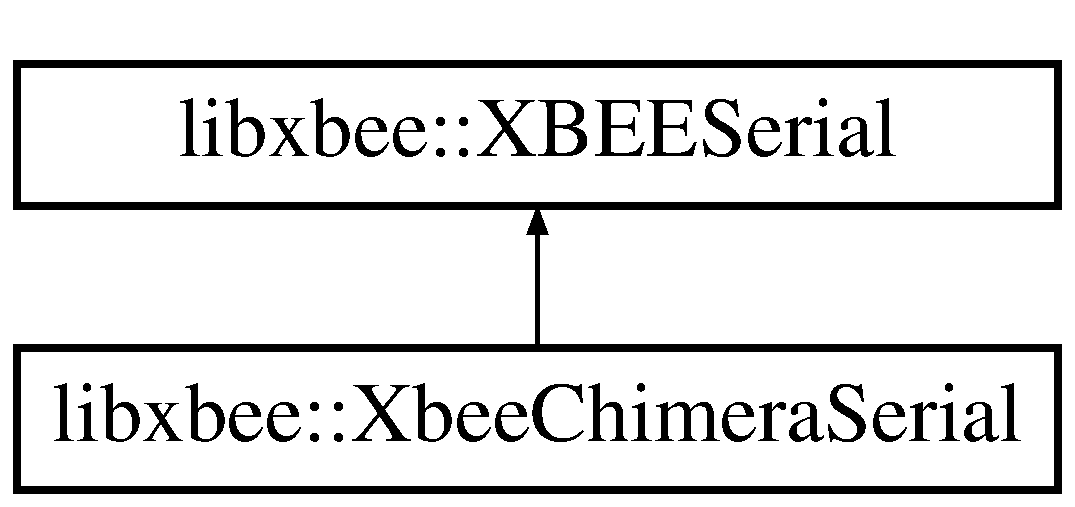
\includegraphics[height=2.000000cm]{classlibxbee_1_1_x_b_e_e_serial}
\end{center}
\end{figure}
\subsection*{Public Member Functions}
\begin{DoxyCompactItemize}
\item 
\mbox{\Hypertarget{classlibxbee_1_1_x_b_e_e_serial_ab18c88d5c4d1ab46f335ba68696fc6b6}\label{classlibxbee_1_1_x_b_e_e_serial_ab18c88d5c4d1ab46f335ba68696fc6b6}} 
virtual void {\bfseries write} (uint8\+\_\+t $\ast$data, size\+\_\+t length)=0
\item 
\mbox{\Hypertarget{classlibxbee_1_1_x_b_e_e_serial_a5044fb4e727f88d19f6c1ce55dd25d20}\label{classlibxbee_1_1_x_b_e_e_serial_a5044fb4e727f88d19f6c1ce55dd25d20}} 
virtual void {\bfseries read} (uint8\+\_\+t $\ast$data, size\+\_\+t length)=0
\end{DoxyCompactItemize}


The documentation for this class was generated from the following file\+:\begin{DoxyCompactItemize}
\item 
xb\+\_\+serial.\+hpp\end{DoxyCompactItemize}

\chapter{File Documentation}
\hypertarget{xb__definitions_8hpp}{}\section{xb\+\_\+definitions.\+hpp File Reference}
\label{xb__definitions_8hpp}\index{xb\+\_\+definitions.\+hpp@{xb\+\_\+definitions.\+hpp}}
\subsection*{Classes}
\begin{DoxyCompactItemize}
\item 
struct \mbox{\hyperlink{structlibxbee_1_1_version}{libxbee\+::\+Version}}
\end{DoxyCompactItemize}
\subsection*{Macros}
\begin{DoxyCompactItemize}
\item 
\mbox{\Hypertarget{xb__definitions_8hpp_a0ee2a4a21a4189e9a9328c3d2183976c}\label{xb__definitions_8hpp_a0ee2a4a21a4189e9a9328c3d2183976c}} 
\#define {\bfseries X\+B\+\_\+\+E\+N\+T\+E\+R\+\_\+\+A\+T\+\_\+\+M\+O\+DE}~\char`\"{}+++\char`\"{}
\item 
\mbox{\Hypertarget{xb__definitions_8hpp_ada3f517fef6beb155ea6dbfc13233e5b}\label{xb__definitions_8hpp_ada3f517fef6beb155ea6dbfc13233e5b}} 
\#define {\bfseries X\+B\+\_\+\+E\+X\+P\+\_\+\+R\+S\+L\+T\+\_\+\+P\+I\+NG}~\char`\"{}O\+K\textbackslash{}r\char`\"{}
\end{DoxyCompactItemize}
\textbf{ }\par
\begin{DoxyCompactItemize}
\item 
\#define \mbox{\hyperlink{group___diagnostic_commands_ga604d8e87718a1dc53cded0e3c020fc40}{X\+B\+\_\+\+F\+I\+R\+M\+W\+A\+R\+E\+\_\+\+V\+ER}}~\char`\"{}VR\char`\"{}
\item 
\#define \mbox{\hyperlink{group___diagnostic_commands_ga58a2fc2812c3b0fd035f22391354ec16}{X\+B\+\_\+\+H\+A\+R\+D\+W\+A\+R\+E\+\_\+\+V\+ER}}~\char`\"{}HV\char`\"{}
\end{DoxyCompactItemize}

\textbf{ }\par
\begin{DoxyCompactItemize}
\item 
\#define \mbox{\hyperlink{group___a_t_command_options_ga44b29b82d01677566af011179946866f}{X\+B\+\_\+\+C\+M\+D\+\_\+\+M\+O\+D\+E\+\_\+\+T\+I\+M\+E\+O\+UT}}~\char`\"{}CT\char`\"{}
\item 
\#define \mbox{\hyperlink{group___a_t_command_options_ga521bbb1db05244aa3171ddeacb3a528e}{X\+B\+\_\+\+C\+M\+D\+\_\+\+M\+O\+D\+E\+\_\+\+E\+X\+IT}}~\char`\"{}CN\char`\"{}
\item 
\#define \mbox{\hyperlink{group___a_t_command_options_ga87806745d2177177af3bc9da86cbdd2f}{X\+B\+\_\+\+S\+E\+T\+\_\+\+G\+U\+A\+R\+D\+\_\+\+T\+I\+ME}}~\char`\"{}GT\char`\"{}
\item 
\#define \mbox{\hyperlink{group___a_t_command_options_gaaa54d14d569183034d941ef1e82dc3e5}{X\+B\+\_\+\+S\+E\+T\+\_\+\+C\+M\+D\+\_\+\+S\+E\+Q\+\_\+\+C\+H\+AR}}~\char`\"{}CC\char`\"{}
\end{DoxyCompactItemize}


%--- End generated contents ---

% Index
\backmatter
\newpage
\phantomsection
\clearemptydoublepage
\addcontentsline{toc}{chapter}{Index}
\printindex

\end{document}
